\newcommand{\D}{6} % number of dimensions (config option)
\newcommand{\U}{7} % number of scale units (config option)

\newdimen\R % maximal diagram radius (config option)
\R=3.5cm
\newdimen\L % radius to put dimension labels (config option)
\L=4.3cm

\newcommand{\A}{360/\D} % calculated angle between dimension axes
\newcommand{\spiderweb}[1]{
  \path (0:0cm) coordinate (O); % define coordinate for origin

  % draw the spiderweb
  \foreach \X in {1,...,\D}{
    \draw (\X*\A:0) -- (\X*\A:\R);
  }

  % the dots on the axis
  \foreach \Y in {0,...,\U}{
    \foreach \X in {1,...,\D}{
      \path (\X*\A:\Y*\R/\U) coordinate (D\X-\Y);
      \fill (D\X-\Y) circle (1pt);
    }

    % this draws the sectors
    \draw [opacity=0.3] (0:\Y*\R/\U) \foreach \X in {1,...,\D}{
      -- (\X*\A:\Y*\R/\U)
    } -- cycle;
  }

  % define labels for each dimension axis (names config option)
  \path (1*\A:\L) node[align=center] (L1) {#1 Minimal Update \\ #1 Overhead};
  \path (2*\A:\L) node[align=center] (L2) {#1 Random \\ #1 Writes};
  \path (3*\A:\L) node[align=center] (L3) {#1 Memory \\ #1 Efficiency};
  \path (4*\A:\L) node[align=center] (L4) {#1 Clearing \\ #1 Efficiency};
  \path (5*\A:\L) node[align=center] (L5) {#1 Sparse Coverage \\ #1 Efficiency};
  \path (6*\A:\L) node[align=center] (L6) {#1 Col. Dect. \\ #1 Throughput};

}

\newcommand{\spiderwebdata}[1]{
  % Voxel lists (blue)
  \draw [fill, opacity=#1, color=blue, line width=1.5pt]
  (D1-1) -- (D2-2) -- (D3-6) -- (D4-6) -- (D5-4) -- (D6-6) -- cycle;

  % Voxel map (red)
  \draw [fill, opacity=#1, color=red, line width=1.5pt]
  (D1-5) -- (D2-6) -- (D3-2) -- (D4-5) -- (D5-1) -- (D6-5) -- cycle;

  % Octree (green)
  \draw [fill, opacity=#1, color=green, line width=1.5pt]
  (D1-2) -- (D2-4) -- (D3-5) -- (D4-3) -- (D5-6) -- (D6-4) -- cycle;
}




\chapter{Umsetzung in GPU-Voxels}
\label{chap:umsetzung_gpu_voxels}


\begin{infobox}{statement}
  \label{def:parallel}
  Für das Design von effizienten Algorithmen ist eine genaue Kenntnis über das Verarbeitungsprinzip der Zielhardware essentiell.
  Da sich GPU und CPU in ihrer Parallelisierung grundlegend Unterscheiden, können CPU Algorithmen die auf SPMD Verarbeitung optimiert sind, abhängig von ihrem Datenmodell gar nicht oder nur mit großem Aufwand zu GPU geigneten SIMD Algorithmen portiert werden.
\end{infobox}

\section{Voxeltypen}
\begin{infobox}{definition}
  \label{def:voxel_types}
  Es wurden mehrere \textbf{Voxel-Typen} implementiert, um unterschiedliche Informationen repräsentieren zu können.
  Dies können Belegtheitswahrscheinlichkeiten, Distanzen oder Bitmuster sein.
  Für jeden Voxel-Typen müssen Operatoren implementiert werden, um seine spezifischen Informationen zu interpretieren.
  Nicht zu verwechseln mit der Voxel-Bedeutung (siehe \cref{def:parallel}).
\end{infobox}
\improvement{Konkrete Anzahl an Voxel-Typen in der Definition angeben. 3?}



\subsubsection{Bitvoxel Kollisionsprüfung}
\label{subsec:bitvoxel_col_tests}


\begin{figure}[!htb]
  \centering
  \tikzstyle{bitlabel} = [font=\footnotesize]
  \begin{tikzpicture}[ auto, node distance=0]
  \node [bit_0] (bit_15) {};
  \node [bit_0, right = of bit_15] (bit_14) {};
  \node [bit_0, right = of bit_14] (bit_13) {};
  \node [bit_0, right = of bit_13] (bit_12) {};
  \node [bit_0, right = of bit_12] (bit_11) {};
  \node [bit_0, right = of bit_11] (bit_10) {};
  \node [bit_1, right = of bit_10] (bit_9) {};
  \node [bit_1, right = of bit_9] (bit_8) {};
  \node [bit_spacer, right = of bit_8] (spacer_0){};
  \node [bit_1, right = of spacer_0] (bit_7) {};
  \node [bit_0, right = of bit_7] (bit_6) {};
  \node [bit_0, right = of bit_6] (bit_5) {};
  \node [bit_0, right = of bit_5] (bit_4) {};
  \node [bit_0, right = of bit_4] (bit_3) {};
  \node [bit_0, right = of bit_3] (bit_2) {};
  \node [bit_1, right = of bit_2] (bit_1) {};
  \node [bit_0, right = of bit_1] (bit_0) {};

  \node [minimum height=1.5em, left = of bit_15] (dots_r) {$\cdots$};
  \node [bitlabel, above = of bit_15] {15};
  \node [bitlabel, above = of bit_8] {8};
  \node [bitlabel, above = of bit_7] {7};
  \node [bitlabel, above = of bit_0] {0};

  \node [below = 7mm of bit_0] (label_occupied) {Belegt};
  \node [below = 7mm of bit_4] (label_sv_start) {SSV-ID 0};
  \node [below = 7mm of bit_9] (label_sv_9) {SSV-ID 5};

  \draw [line] (label_occupied) -- (bit_1);
  \draw [line] (label_sv_start) -- (bit_4);
  \draw [line] (label_sv_9) -- (bit_9);
  \end{tikzpicture}
  \caption{Die ersten beiden Bytes aus dem Bitvektors eines Voxels, der zu drei Zeitschritten belegt ist (vgl. grünes Volumen aus \cref{subsec:bitvoxel_col_tests}).
    Alle nicht dargestellten Bits des Vektors sind nicht gesetzt.}
  \label{fig:bitvector_example}
\end{figure}

\begin{figure}[!htb]
  \centering
  \tikzstyle{bitlabel} = [font=\footnotesize]
\begin{tikzpicture}[ auto, node distance=0]
	\node [bit_0_green] (bit_23_r) {};
	\node [bit_0_green, right = of bit_23_r] (bit_22_r) {};
	\node [bit_0_green, right = of bit_22_r] (bit_21_r) {};
	\node [bit_0_green, right = of bit_21_r] (bit_20_r) {};
	\node [bit_0_green, right = of bit_20_r] (bit_19_r) {};
	\node [bit_0_green, right = of bit_19_r] (bit_18_r) {};
	\node [bit_0_green, right = of bit_18_r] (bit_17_r) {};
	\node [bit_0_green, right = of bit_17_r] (bit_16_r) {};
	\node [bit_spacer, right = of bit_16_r] (spacer_1){};
	\node [bit_0_green, right = of spacer_1] (bit_15_r) {};
	\node [bit_0_green, right = of bit_15_r] (bit_14_r) {};
	\node [bit_0_green, right = of bit_14_r] (bit_13_r) {};
	\node [bit_1_green, right = of bit_13_r] (bit_12_r) {};
	\node [bit_1_green, right = of bit_12_r] (bit_11_r) {};
	\node [bit_1_green, right = of bit_11_r] (bit_10_r) {};
	\node [bit_1_green, right = of bit_10_r] (bit_9_r) {};
	\node [bit_1_green, right = of bit_9_r] (bit_8_r) {};
	\node [bit_spacer, right = of bit_8_r] (spacer_0){};
	\node [bit_1_green, right = of spacer_0] (bit_7_r) {};
	\node [bit_1_green, right = of bit_7_r] (bit_6_r) {};
	\node [bit_1_green, right = of bit_6_r] (bit_5_r) {};
	\node [bit_1_green, right = of bit_5_r] (bit_4_r) {};
	\node [bit_1_green, right = of bit_4_r] (bit_3_r) {};
	\node [bit_1_green, right = of bit_3_r] (bit_2_r) {};
	\node [bit_0_green, right = of bit_2_r] (bit_1_r) {};
	\node [bit_0_green, right = of bit_1_r] (bit_0_r) {};
	\node [right = of bit_0_r] (dots_r_0) {$\cdots$};
	\node [minimum height=1.5em, left = of bit_23_r] (dots_r) {$\cdots$};
	\node [minimum height=1.5em, left = of dots_r] (label_r) {Roboter};

	\node [bit_0_green, below = 3mm of bit_23_r] (bit_23_o) {};
	\node [bit_0_green, right = of bit_23_o] (bit_22_o) {};
	\node [bit_0_green, right = of bit_22_o] (bit_21_o) {};
	\node [bit_0_green, right = of bit_21_o] (bit_20_o) {};
	\node [bit_0_green, right = of bit_20_o] (bit_19_o) {};
	\node [bit_0_green, right = of bit_19_o] (bit_18_o) {};
	\node [bit_1_green, right = of bit_18_o] (bit_17_o) {};
	\node [bit_1_green, right = of bit_17_o] (bit_16_o) {};
	\node [bit_spacer, right = of bit_16_o] (spacer_1){};
	\node [bit_1_green, right = of spacer_1] (bit_15_o) {};
	\node [bit_1_green, right = of bit_15_o] (bit_14_o) {};
	\node [bit_1_green, right = of bit_14_o] (bit_13_o) {};
	\node [bit_1_green, right = of bit_13_o] (bit_12_o) {};
	\node [bit_1_green, right = of bit_12_o] (bit_11_o) {};
	\node [bit_1_green, right = of bit_11_o] (bit_10_o) {};
	\node [bit_0_green, right = of bit_10_o] (bit_9_o) {};
	\node [bit_0_green, right = of bit_9_o] (bit_8_o) {};
	\node [bit_spacer, right = of bit_8_o] (spacer_0){};
	\node [bit_0_green, right = of spacer_0] (bit_7_o) {};
	\node [bit_0_green, right = of bit_7_o] (bit_6_o) {};
	\node [bit_0_green, right = of bit_6_o] (bit_5_o) {};
	\node [bit_0_green, right = of bit_5_o] (bit_4_o) {};
	\node [bit_0_green, right = of bit_4_o] (bit_3_o) {};
	\node [bit_0_green, right = of bit_3_o] (bit_2_o) {};
	\node [bit_0_green, right = of bit_2_o] (bit_1_o) {};
	\node [bit_0_green, right = of bit_1_o] (bit_0_o) {};
	\node [right = of bit_0_o] (dots_o_0) {$\cdots$};
	\node [minimum height=1.5em, left = of bit_23_o] (dots_o) {$\cdots$};
	\node [minimum height=1.5em, left = of dots_o] (label_obst) {Hindernis};

	\node [bit_0, below = 3mm of bit_23_o] (bit_23_and) {};
	\node [bit_0, right = of bit_23_and] (bit_22_and) {};
	\node [bit_0, right = of bit_22_and] (bit_21_and) {};
	\node [bit_0, right = of bit_21_and] (bit_20_and) {};
	\node [bit_0, right = of bit_20_and] (bit_19_and) {};
	\node [bit_0, right = of bit_19_and] (bit_18_and) {};
	\node [bit_0, right = of bit_18_and] (bit_17_and) {};
	\node [bit_0, right = of bit_17_and] (bit_16_and) {};
	\node [bit_spacer, right = of bit_16_and] (spacer_1){};
	\node [bit_0, right = of spacer_1] (bit_15_and) {};
	\node [bit_0, right = of bit_15_and] (bit_14_and) {};
	\node [bit_0, right = of bit_14_and] (bit_13_and) {};
	\node [bit_1, right = of bit_13_and] (bit_12_and) {};
	\node [bit_1, right = of bit_12_and] (bit_11_and) {};
	\node [bit_1, right = of bit_11_and] (bit_10_and) {};
	\node [bit_0, right = of bit_10_and] (bit_9_and) {};
	\node [bit_0, right = of bit_9_and] (bit_8_and) {};
	\node [bit_spacer, right = of bit_8_and] (spacer_0){};
	\node [bit_0, right = of spacer_0] (bit_7_and) {};
	\node [bit_0, right = of bit_7_and] (bit_6_and) {};
	\node [bit_0, right = of bit_6_and] (bit_5_and) {};
	\node [bit_0, right = of bit_5_and] (bit_4_and) {};
	\node [bit_0, right = of bit_4_and] (bit_3_and) {};
	\node [bit_0, right = of bit_3_and] (bit_2_and) {};
	\node [bit_0, right = of bit_2_and] (bit_1_and) {};
	\node [bit_0, right = of bit_1_and] (bit_0_and) {};
	\node [right = of bit_0_and] (dots_and_0) {$\cdots$};
	\node [minimum height=1.5em, left = of bit_23_and] (dots_and) {$\cdots$};
	\node [minimum height=1.5em, left = of dots_and] (label_and) {UND};
	
	\node [bit_0, below = 3mm of bit_23_and] (bit_23_and5) {};
	\node [bit_0, right = of bit_23_and5] (bit_22_and5) {};
	\node [bit_0, right = of bit_22_and5] (bit_21_and5) {};
	\node [bit_0, right = of bit_21_and5] (bit_20_and5) {};
	\node [bit_0, right = of bit_20_and5] (bit_19_and5) {};
	\node [bit_0, right = of bit_19_and5] (bit_18_and5) {};
	\node [bit_1, right = of bit_18_and5] (bit_17_and5) {};
	\node [bit_1, right = of bit_17_and5] (bit_16_and5) {};
	\node [bit_spacer, right = of bit_16_and5] (spacer_1){};
	\node [bit_1, right = of spacer_1] (bit_15_and5) {};
	\node [bit_1, right = of bit_15_and5] (bit_14_and5) {};
	\node [bit_1, right = of bit_14_and5] (bit_13_and5) {};
	\node [bit_1, right = of bit_13_and5] (bit_12_and5) {};
	\node [bit_1, right = of bit_12_and5] (bit_11_and5) {};
	\node [bit_1, right = of bit_11_and5] (bit_10_and5) {};
	\node [bit_1, right = of bit_10_and5] (bit_9_and5) {};
	\node [bit_1, right = of bit_9_and5] (bit_8_and5) {};
	\node [bit_spacer, right = of bit_8_and5] (spacer_0){};
	\node [bit_1, right = of spacer_0] (bit_7_and5) {};
	\node [bit_1, right = of bit_7_and5] (bit_6_and5) {};
	\node [bit_1, right = of bit_6_and5] (bit_5_and5) {};
	\node [bit_0, right = of bit_5_and5] (bit_4_and5) {};
	\node [bit_0, right = of bit_4_and5] (bit_3_and5) {};
	\node [bit_0, right = of bit_3_and5] (bit_2_and5) {};
	\node [bit_0, right = of bit_2_and5] (bit_1_and5) {};
	\node [bit_0, right = of bit_1_and5] (bit_0_and5) {};
	\node [right = of bit_0_and5] (dots_and5_0) {$\cdots$};
	\node [minimum height=1.5em, left = of bit_23_and5] (dots_and5) {$\cdots$};
	\node [minimum height=1.5em, left = of dots_and5] (label_and5) {UND\_5};

	\node [bit_0_red, below = 3mm of bit_23_and5] (bit_23_res) {};
	\node [bit_0_red, right = of bit_23_res] (bit_22_res) {};
	\node [bit_0_red, right = of bit_22_res] (bit_21_res) {};
	\node [bit_0_red, right = of bit_21_res] (bit_20_res) {};
	\node [bit_0_red, right = of bit_20_res] (bit_1_red9_res) {};
	\node [bit_0_red, right = of bit_1_red9_res] (bit_1_red8_res) {};
	\node [bit_0_red, right = of bit_1_red8_res] (bit_1_red7_res) {};
	\node [bit_0_red, right = of bit_1_red7_res] (bit_1_red6_res) {};
	\node [bit_spacer, right = of bit_1_red6_res] (spacer_1){};
	\node [bit_0_red, right = of spacer_1] (bit_1_red5_res) {};
	\node [bit_0_red, right = of bit_1_red5_res] (bit_1_red4_res) {};
	\node [bit_0_red, right = of bit_1_red4_res] (bit_1_red3_res) {};
	\node [bit_1_red, right = of bit_1_red3_res] (bit_1_red2_res) {};
	\node [bit_1_red, right = of bit_1_red2_res] (bit_1_red1_res) {};
	\node [bit_1_red, right = of bit_1_red1_res] (bit_1_red0_res) {};
	\node [bit_1_red, right = of bit_1_red0_res] (bit_9_res) {};
	\node [bit_1_red, right = of bit_9_res] (bit_8_res) {};
	\node [bit_spacer, right = of bit_8_res] (spacer_0){};
	\node [bit_1_red, right = of spacer_0] (bit_7_res) {};
	\node [bit_1_red, right = of bit_7_res] (bit_6_res) {};
	\node [bit_1_red, right = of bit_6_res] (bit_5_res) {};
	\node [bit_0_red, right = of bit_5_res] (bit_4_res) {};
	\node [bit_0_red, right = of bit_4_res] (bit_3_res) {};
	\node [bit_0_red, right = of bit_3_res] (bit_2_res) {};
	\node [bit_0_red, right = of bit_2_res] (bit_1_red_res) {};
	\node [bit_0_red, right = of bit_1_red_res] (bit_0_red_res) {};
	\node [right = of bit_0_red_res] (dots_res_0) {$\cdots$};
	\node [minimum height=1.5em, left = of bit_23_res] (dots_res) {$\cdots$};
	\node [minimum height=1.5em, left = of dots_res] (label_res) {Ergebnis};


	\node [bitlabel, above = of bit_23_r] {31};
	\node [bitlabel, above = of bit_16_r] {24};
	\node [bitlabel, above = of bit_15_r] {23};
	\node [bitlabel, above = of bit_8_r] {16};
	\node [bitlabel, above = of bit_2_r] {10};


\end{tikzpicture}
  \caption[Beispiel der Kollisionserkennung]{Beispiel der Kollisionserkennung zwischen dem \Gls{SV} Bitvektor eines Roboters und eines Hindernisses aus \citestudthesis{mauch15}.
    Die Bitvektoren von Roboter und Hindernis sind in grün dargestellt, das Ergebnis der Kollisionsprüfung in rot.}
  \label{fig:bitvector_collision}
\end{figure}


\section{Datenstrukturen und spezifische Strategien zur Befüllung und Daten-Extraktion}

% {#1 Minimal Update Overhead};
% {#2 Random Writes};
% {#3 Memory Efficiency};
% {#4 Clearing Efficiency};
% {#5 Sparse Coverage Efficiency};
% {#6 Col.Dect. Throughput};


\begin{figure*}[htbp]
    \centering
    \subcaptionbox{Umgebungskarte\label{subfigure:spiderweb:EnvironmentMap}}[.5\textwidth]{
      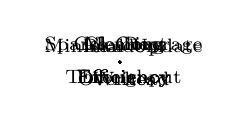
\begin{tikzpicture}[scale=0.5]
      \spiderweb{\scriptsize}
      \spiderwebdata{0.3}
      % A priori Environment Map
      \draw [opacity=0.8, color=black, densely dashed, line width=0.7pt]
      (D1-2) -- (D2-3) -- (D3-5) -- (D4-2) -- (D5-5) -- (D6-4) -- cycle;
      \end{tikzpicture}
    }%
  \subcaptionbox{Roboter oder dynamisches Hindernis\label{subfigure:spiderweb:RobotMap}}[.5\textwidth]{
    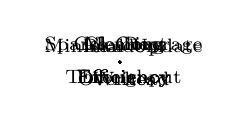
\begin{tikzpicture}[scale=0.5]
    \spiderweb{\scriptsize}
    \spiderwebdata{0.3}
    % Robot Map and Dynamic Obstacles
    \draw [opacity=0.8, color=black, densely dashed, line width=0.7pt]
    (D1-5) -- (D2-5) -- (D3-2) -- (D4-5) -- (D5-5) -- (D6-5) -- cycle;
    \end{tikzpicture}
  } \\
  \subcaptionbox{Swept Volumen\label{subfigure:spiderweb:SweptVolumes}}[.5\textwidth]{
     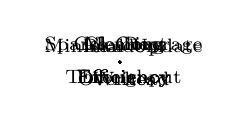
\begin{tikzpicture}[scale=0.5]
     \spiderweb{\scriptsize}
     \spiderwebdata{0.3}
     % Swept volumes
     \draw [opacity=0.8, color=black, densely dashed, line width=0.7pt]
     (D1-3) -- (D2-5) -- (D3-3) -- (D4-5) -- (D5-3) -- (D6-5) -- cycle;
     \end{tikzpicture}
  }%
  \subcaptionbox{Bewegungsprimitiv\label{subfigure:spiderweb:MotionPrimitives}}[.5\textwidth]{
    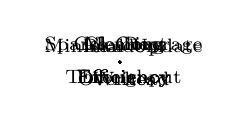
\begin{tikzpicture}[scale=0.5]
    \spiderweb{\scriptsize}
    \spiderwebdata{0.3}
    % Motion Primiives map
    \draw [opacity=0.8, color=black, densely dashed, line width=0.7pt]
    (D1-3) -- (D2-2) -- (D3-5) -- (D4-5) -- (D5-4) -- (D6-5) -- cycle;
    \end{tikzpicture}
  }%
    \caption{Comparison of the requirements of different data characteristics from our use cases (black dashed outline) against the implemented storage structures: Voxel map (red), Octree (green) and voxel lists (blue). Compare \cref{fig:spiderweb}.}
  \label{fig:SpiderWebComparisonOfData}
\end{figure*}


\begin{figure}[h]
 \centering
  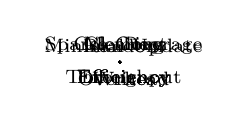
\begin{tikzpicture}[scale=0.5]
    \spiderweb{\scriptsize}
    \spiderwebdata{0.4}
  \end{tikzpicture}
  \caption{Properties of the implemented storage structures that can be matched to the use cases from \cref{fig:SpiderWebComparisonOfData}:
  Voxel map (red), Octree (green), voxel lists (blue)}
  \label{fig:spiderweb}
\end{figure}



\subsubsection{Offset Translation}
\label{subsec:offset_translation}
Soll die Punktewolke eines mobilen Objektes mit einer Voxelmap geschnitten werden, kann im Falle einer rein translatorischen Bewegung auf die Transformation der Punktewolke verzichtet werden.
In diesem Fall kann die Punktewolke einmalig in eine Voxelmap oder Voxelliste eingetragen werden und die Translation mittels der \cref{eqn:voxelmap_diskretisierung} auf einen Offset abgebildet werden.
Bei einer Kollisionsprüfung wird dieser Offset auf die Basis-Adresse der ortsfesten Voxelmap addiert, und somit die Datenstruktur des mobilen Objektes virtuell verschoben.

\begin{figure}[!htb]
  \centering
  \begin{subfigure}[b][][c]{0.5\textwidth}\centering
    \centering
    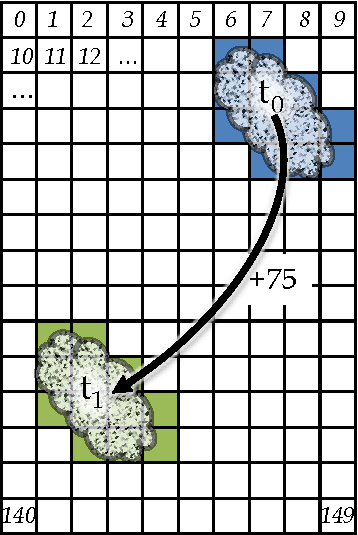
\includegraphics[width=0.8\textwidth]{04_images/3d_representation/offset_translation.pdf}
    \subcaption{Addressierungsschema der Voxelliste}\label{subfig:offset_translation_grid}
  \end{subfigure}%
  \begin{subtable}[b][][c]{0.5\textwidth}
    \centering
    \pgfplotstableset{
      create on use/w_offset/.style={create col/expr ={\thisrow{voxel_id}+75}},
      create on use/the_offset/.style={create col/set list={\multirow{12}{2cm}[0pt]{\enspace\quad +75}} }
    }

    \pgfplotstabletypeset[
    col sep=tab,
    columns={voxel_id,the_offset,w_offset},
    columns/voxel_id/.style={column name= $t_0$, column type={c}},
    columns/the_offset/.style={string type, column name=Offset, column type={c}},
    columns/w_offset/.style={column name= $t_1$, column type={c}},
    every head row/.style={
      before row={\toprule \multicolumn{3}{c}{\bfseries Voxel-IDs} \\ \cmidrule(lr){1-3} },
      after row=\cmidrule(lr){1-1} \cmidrule(lr){2-2} \cmidrule(lr){3-3}
    },
    every last row/.style={after row=\bottomrule},
    ]{04_images/3d_representation/offset_example.csv}
    \subcaption{Voxelliste vor und nach Translation}\label{subfig:offset_translation_lists}
  \end{subtable}
  \caption{Translation der Voxelliste einer voxelisierten Punktewolke zwischen $t_0$ und $t_1$. Alle Voxel-IDs der Liste werden um den Versatz inkrementiert. Dies erspart die geometrische Transformation der Punktewolke.}
  \label{fig:offset_translation}

\end{figure}



\todo[inline]{Machen Probab Voxellisten Sinn? Wie Updaten (incr decr probab)?}



\section{Visualisierung}
\label{sec:visualization}

Da Voxel eine sehr einfache Würfelgeometrie aufweisen und ihre Eigenschaften beziehungsweise Zugehörigkeiten über Farben darstellbar sind, besteht die Herausforderung nicht in der Art der Darstellung, sonder in der Effizienz und der Menge der darzustellenden Voxel.
Im Gegensatz zu weit verbreiteten Grafik-Engines, wie \textit{OGRE}\footnote{\url{http://www.ogre3d.org/}} oder Spiele-Engines wie beispielsweise die \textit{Cryengine}\footnote{\url{http://cryengine.com/}} benötigt die Visualisierung für Voxel entsprechend keinen komplexen Szenengraphen, aufwendige Licht- oder Textureffekte.

Eine erste Implementierung basierte darauf, Kopien aller darzustellenden Informationen, die auf dem \textit{\Gls{Device}} nach einer Berechnung vorlagen, auf den \textit{\Gls{Host}} zu kopieren, dort in \Gls{OpenGL} Strukturen umzuwandeln, und diese dann erneut auf die \Gls{GPU} zu transferieren, um sie anzuzeigen (siehe \cref{subfig:viz_overhead}).
Wie in \cref{subsec:cuda_contextswitch} beschrieben, stellt dieses mehrfache Kopieren ein Performanceproblem dar.

Dieser Ansatz wurde in der Bachelorarbeit~\citestudthesis{wagner14} von Matthias Wagner erfolgreich umgesetzt und über die Dauer der Dissertation ständig weiterentwickelt.
Alle Voxel-Grafiken in diesem Dokument, mit Ausnahme derer in \cref{sec:rot_mp_planning}, wurden mit dieser Visualisierung erstellt.





\subsubsection{Supervoxel}
\missingfigure{Scan in unterschiedlichen Supervoxel-Auflösungen}



\subsection{Sortieren der Voxeltypen}

\todo{Convert to Booktabs}


\begin{figure}
  \begin{tikzpicture}
  \begin{axis}[ymin=0, ymax=350,xmin=0, xmax = 33,
  xlabel={Supervoxel-Größe},
  ylabel={Frames pro Sekunde},
  width=0.6\textwidth,
  legend style={at ={(1.8,0.8)}, legend columns=1}
  ]
  \addlegendimage{empty legend}
  \addlegendimage{empty legend}
  \addplot[very thick, color = black] table[x=svoxel, y=fps_w]
  {04_images/gpu_visualization/performance_view.csv};
  \addplot[very thick, color = black,dashdotdotted] table[x=svoxel, y=fps_v]
  {04_images/gpu_visualization/performance_view.csv};
  \addlegendentry{\hspace{-1.0cm}\textbf{Frames / Sekunde}}
  \addlegendentry{}
  \addlegendentry{nicht beschränkt}
  \addlegendentry{beschränkt}
  \end{axis}
  \begin{axis}[ymin=0, ymax=61000,xmin=0, xmax = 33,
  axis y line*=right,
  xticklabels={,,},
  ylabel={Gezeichnete Voxel},
  every axis y label/.append style ={RedViolet},
  every tick label/.append style={RedViolet},
  width=0.6\textwidth,
  legend style={at ={(1.8,0.45)}, legend columns=1}
  ]
  \addlegendimage{empty legend}
  \addlegendimage{empty legend}
  \addplot[very thick, color = RedViolet] table[x=svoxel, y=voxel_w]
  {04_images/gpu_visualization/performance_view.csv};
  \addplot[very thick, color = RedViolet,dashdotdotted] table[x=svoxel, y=voxel_v]
  {04_images/gpu_visualization/performance_view.csv};
  \addlegendentry[RedViolet]{\hspace{-0.8cm}\textbf{Gezeichnete Voxel}}
  \addlegendentry{}
  \addlegendentry{nicht beschränkt}
  \addlegendentry{beschränkt}
  \end{axis}
  \end{tikzpicture}
  \caption[Anstieg der Bildrate bei Einschränkung des Sichtbereiches]{Anstieg der Bildrate bei Einschränkung des Sichtbereiches (Szene aus \cref{fig:visualization_benchmark_culling}). Daten aus~\citestudthesis{wagner14}).}
  \label{fig:visualization_benchmark_culling}
\end{figure}


\begin{figure}[h]

  \begin{subtable}[c]{0.5\textwidth}
    \pgfplotstabletypeset[
    col sep=tab,
    string type,
    columns={seitenlaenge,dimension,anzahlVoxel},
    columns/anzahlVoxel/.style={column name=\; Voxel \;, column type={c}},
    columns/dimension/.style={column name= Dimension, column type={c}},
    columns/seitenlaenge/.style={column name= $\textrm{[cm]}$, column type={c}},
    every head row/.style={before row={\toprule Seiten- \\länge & Voxelmap & Anzahl \\ },
      after row=\cmidrule(lr){1-3}},
    every last row/.style={after row=\bottomrule},
    ]{04_images/gpu_visualization/without_gigantic_map.csv}
  \end{subtable}
  ~
  \begin{subfigure}[c][][c]{0.5\textwidth}\centering
    \begin{tikzpicture}
    \begin{axis}[ymin=0, ymax=80,xmin=007, xmax = 21,
    xlabel={Voxel Seitenlänge $\textrm{[cm]}$  },
    ylabel={Bildrate},
    width=1.0\textwidth,
    legend style={at ={(1.0,1.0)}, legend columns=1},
    scaled ticks =false
    ]
    \addplot[very thick, color = Aquamarine,mark=x] table[x=seitenlaenge, y=fps,col sep=tab]
    {04_images/gpu_visualization/without_gigantic_map.csv};
    \end{axis}
    \end{tikzpicture}
  \end{subfigure}
  \caption[Erreichte Bildraten bei der Visualisierung umfangreichen Daten]{Erreichte Bildraten bei der Visualisierung umfangreichen Daten (siehe \cref{fig:visualization_fzi_map}) mit unterschiedlichen Voxel-Seitenlängen.}
  \label{fig:visualization_fzi_map}
\end{figure}
